
%% The first command in your LaTeX source must be the \documentclass command.
\documentclass[sigconf]{acmart}
%% \BibTeX command to typeset BibTeX logo in the docs
\AtBeginDocument{%
  \providecommand\BibTeX{{%
    \normalfont B\kern-0.5em{\scshape i\kern-0.25em b}\kern-0.8em\TeX}}}

%% Rights management information.  This information is sent to you
%% when you complete the rights form.  These commands have SAMPLE
%% values in them; it is your responsibility as an author to replace
%% the commands and values with those provided to you when you
%% complete the rights form.
\setcopyright{acmcopyright}
\copyrightyear{2021}
\acmYear{2021}
\acmDOI{TO BE DETERMINED}

%% These commands are for a PROCEEDINGS abstract or paper.
\acmConference[ICAIL '21]{Proceedings of the 18th International Conference on Artificial Intelligence and Law}{June 28-30, 2021}{Sao Paulo, Brazil}
\acmBooktitle{Proceedings of the 18th International Conference on Artificial Intelligence and Law, June 28-30, 2021, Sao Paulo, Brazil}
\acmPrice{TBD}
\acmISBN{TBD}


%%
%% Submission ID.
%% Use this when submitting an article to a sponsored event. You'll
%% receive a unique submission ID from the organizers
%% of the event, and this ID should be used as the parameter to this command.
\acmSubmissionID{TBD}

%%
%% The majority of ACM publications use numbered citations and
%% references.  The command \citestyle{authoryear} switches to the
%% "author year" style.
%%
%% If you are preparing content for an event
%% sponsored by ACM SIGGRAPH, you must use the "author year" style of
%% citations and references.
%% Uncommenting
%% the next command will enable that style.
%%\citestyle{acmauthoryear}

%%
%% end of the preamble, start of the body of the document source.

\usepackage{listings}
\lstdefinestyle{mystyle}{
    basicstyle=\ttfamily\footnotesize,
    breakatwhitespace=false,         
    breaklines=true,                 
    captionpos=b,                    
    keepspaces=true,                  
    numbersep=5pt,                  
    showspaces=false,                
    showstringspaces=false,
    showtabs=false,                  
    tabsize=2
}

\lstset{style=mystyle}

\begin{document}

%%
%% The "title" command has an optional parameter,
%% allowing the author to define a "short title" to be used in page headers.
\title{Constrained Answer Set Programming as a Tool to Improve Legislative Drafting}
\subtitle{A Rules as Code Experiment}

%%
%% The "author" command and its associated commands are used to define
%% the authors and their affiliations.
%% Of note is the shared affiliation of the first two authors, and the
%% "authornote" and "authornotemark" commands
%% used to denote shared contribution to the research.
\author{Jason Morris}
\email{jmorris@smu.edu.sg}
\orcid{???}
\affiliation{%
  \institution{Singapore Management University Centre for Computational Law}
  \streetaddress{Armenian Street}
  \city{Singapore}
  \state{Singapore}
  \country{Singapore}
  \postcode{123456}
}

%%
%% By default, the full list of authors will be used in the page
%% headers. Often, this list is too long, and will overlap
%% other information printed in the page headers. This command allows
%% the author to define a more concise list
%% of authors' names for this purpose.
%%\renewcommand{\shortauthors}{Trovato and Tobin, et al.}

%%
%% The abstract is a short summary of the work to be presented in the
%% article.
\begin{abstract}
  The paper presents an interdicsiplinary experiment to determine whether
  the s(CASP) constrained answer set programming languages is an appropriate
  tool for use in Rules as Code, to improve legislative drafting quality.
  Rules as Code, a computer-assisted legislative
  drafting methodology, is briefly introduced. The experiment encodes a section
  of Singapore statute law, revealing a drafting
  error. The paper proposes an amendment to the law and uses the encoding to demonstrate that this amendment would resolve the drafting error.
  The paper concludes that answer set programming with
  justifications is an extremely valuable approach for the drafting phase of
  Rules as Code.
\end{abstract}

%%
%% The code below is generated by the tool at http://dl.acm.org/ccs.cfm.
%% Please copy and paste the code instead of the example below.
%%
\begin{CCSXML}
<ccs2012>
 <concept>
  <concept_id>10010520.10010553.10010562</concept_id>
  <concept_desc>Computer systems organization~Embedded systems</concept_desc>
  <concept_significance>500</concept_significance>
 </concept>
 <concept>
  <concept_id>10010520.10010575.10010755</concept_id>
  <concept_desc>Computer systems organization~Redundancy</concept_desc>
  <concept_significance>300</concept_significance>
 </concept>
 <concept>
  <concept_id>10010520.10010553.10010554</concept_id>
  <concept_desc>Computer systems organization~Robotics</concept_desc>
  <concept_significance>100</concept_significance>
 </concept>
 <concept>
  <concept_id>10003033.10003083.10003095</concept_id>
  <concept_desc>Networks~Network reliability</concept_desc>
  <concept_significance>100</concept_significance>
 </concept>
</ccs2012>
\end{CCSXML}

\ccsdesc[500]{Computer systems organization~Embedded systems}
\ccsdesc[300]{Computer systems organization~Redundancy}
\ccsdesc{Computer systems organization~Robotics}
\ccsdesc[100]{Networks~Network reliability}

%%
%% Keywords. The author(s) should pick words that accurately describe
%% the work being presented. Separate the keywords with commas.
\keywords{legal knowledge representation and reasoning, constraint answer set programming, rules as code}

%% A "teaser" image appears between the author and affiliation
%% information and the body of the document, and typically spans the
%% page.
%%\begin{teaserfigure}
%%  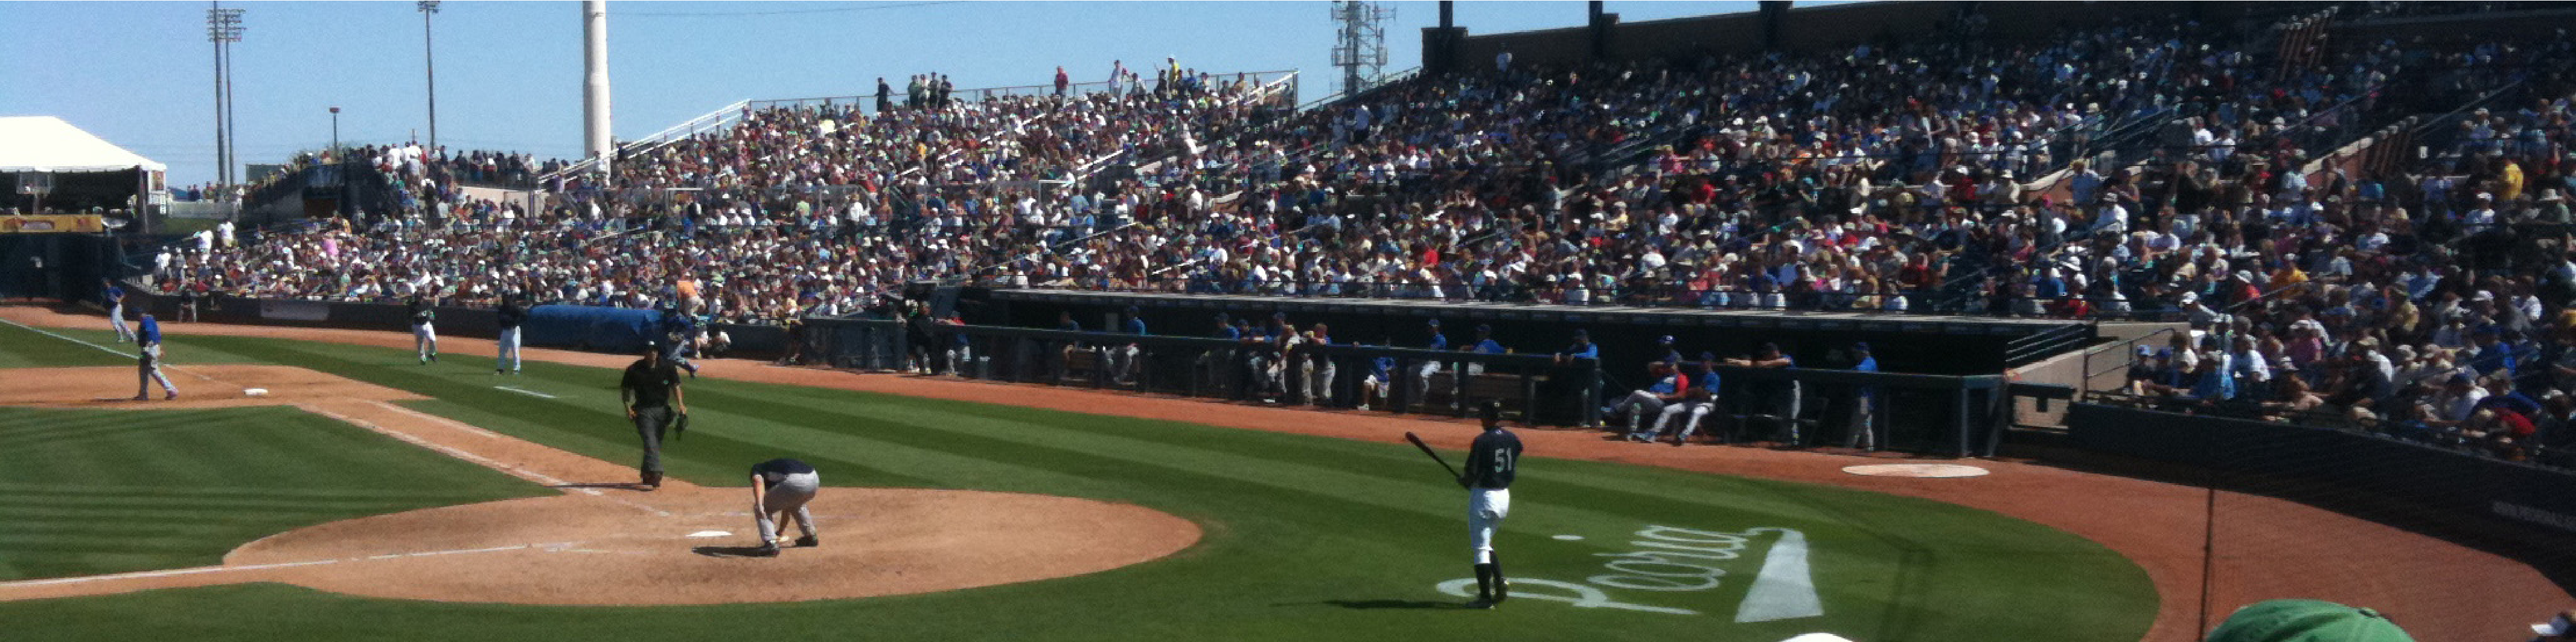
\includegraphics[width=\textwidth]{sampleteaser}
%%  \caption{Seattle Mariners at Spring Training, 2010.}
%%  \Description{Enjoying the baseball game from the third-base
%%  seats. Ichiro Suzuki preparing to bat.}
%%  \label{fig:teaser}
%%\end{teaserfigure}

%%
%% This command processes the author and affiliation and title
%% information and builds the first part of the formatted document.
\maketitle

\section{Introduction}
The Singapore Managment University Centre for Computational Law is conducting research into the development
of a domain-specific language for encoding knowledge about legal rules including legislation, regulation,
and contracts. One of the anticipated use-cases of that language, entitled L4, is for use in Rules as Code.
In pursuit of that objective we are conducting experiments designed to ascertain the practical benefits
of various approaches to symbolic artificial intelligence in the domain of legislation and contract. This paper describes one such experiment.

This paper briefly introduces the concept of Rules as Code, which is an interdisciplinary approach utilizing legal knowledge representation and reasoning to improve drafting quality and simplify the automation of legislation and regulation. It then briefly introduces the tool used in our experiment, s(CASP),
which is a constrained answer set programming (CASP) language, and our motivations for selecting it, which include
the ability to automatically generate explanations for conclusions.
Our use case, section 34 of the Singapore Legal Profession (Professional Conduct) Rules 2015, is then introduced.

The paper then provides a narrative illustration of how we used
s(CASP) in an interdisciplinary setting to discover and
repair problems with legislation. We then report the researcher's impressions
as to the benefits and weaknesses of s(CASP) as compared to other methods for use in the
drafting phase of a Rules as Code process. The paper concludes that justified
answer set programming is extremely valuable to the task of legislative drafting
in the Rules as Code process.

The paper concludes with a brief review of similar work, and ways in which this research could
be extended. We believe that this is the first published use of justified answer
set programming in legal reasoning, and the first published demonstration of the
use of symbolic AI as a tool for use in Rules as Code. 

\section{Rules as Code}

"Rules as Code" in this paper is used to refer to a proposed methodology of legislative and regulatory
drafting. The suggestion that legislation can and should be automated is not new, neither is the idea
that symbolic artificial intelligence approaches are particularly well-suited to the task of representing legal knowledge.

What the Rules as Code proposal changes is the purpose to which these tools are put.
Rather than attempting to encode an existing law, Rules as Code
proposes that these tools should be used at the time of drafting.

This changes the target of the use of the tool from an encoding of the meaning
of the legislation to merely a faithful encoding of the text. The intent of the
drafters is encoded - with the drafters in the room - in the form of tests.
Instead of encoding uncertain guesses at drafters' intent, the encoded and natural 
language version of the legislation are manipulated until they
match each other, and pass those tests.

Rules as Code is inherently interdisciplinary, and requires the addition of
legal knowledge representation and reasoning capabilities to the drafting team.
The anticipated outcomes include improved legislative drafting quality. The attempt
to encode legislative text, and the opportunity to test it automatically, will
reveal errors, inconsistencies, and under-specifications that would not otherwise
have been visible to the drafters. If published, which advocates of Rules as Code
recommend, the encoding can be used
to simplify the automation of compliant legal services, benefiting public
administration, reducing the costs of compliance, and enhancing access to justice. 
The benefits of testability also extend to the
purposes for which the drafting is performed, such as policy design. The encoding 
can be used, for example, to do automated impact assessments of proposed legislative amendments.

This last use is the one which has seen the most real-world adoption thus far,
particularly in France, which has mandated impact assessments with
regard to certain forms of legislation.
The French government has invested in the development of a
programming language, Catala, for use in these purposes.
The OpenFisca library has also been used to
generate the LexImpact service of the French National Assembly, which provides 
legislators and the public
with information about how proposed tax amendments will affect individuals and 
populations.

Despite the development of a small number of tools for Rules as
Code, and the parallel development of a number of tools with similar purposes
aimed at
use in smart contracts, 
there is no widespread agreement on the types of technologies
that are appropriate for use in Rules as Code, and why. The academic conversation
about the strenghts and weaknesses of different technologies with regard to the
task of legislative drafting, as distinct from legal knowledge representation,
has not yet begun. This paper seeks to begin it.

This is a brief introduction, for more information on Rules as Code, the reader is referred to the OECD OPSI
report, "Cracking the Code" published in 2020.

\section{s(CASP)}

s(CASP) is a re-implementation of s(ASP) adding constraints to the answer set programming methods, implemented
in the Ciao programming language.

s(CASP) was selected as a language for use in this experiment because of a number of features that were anticipated to fit these needs of the automation of legal
services. Primary among them is the fact that s(CASP) is capable of generating natural language explanations for its conclusions.
While the value of backtracking explanations has primarily been with regard to
debugging, as in expert system development the rules have traditionally not
represented information that was pertinent to the end users, precisely the opposite
is true with regard to the automation of legal services. The ability to generate
an explanation that tracks, section-by-section, through the text of a legislative
statute is extremely valuable to both the developers and the users of automated
legal services.

s(CASP) also features higher-order logic programming features, the ability
to easily obtain both deductive and abductive reasoning from the same ruleset, and
constraint programming features. Combined, these allow for approaches to defeasibility
that enhance the maintainability of encodings, and for the implementation of
abstractions such as Event Calculus, to allow for the automation of reasoning about
steps taken over time in legal processes.

\section{Section 34, Singapore Legal Profession (Professional Standards) Rules 2015}

Section 34 of the Singapore Legal Profession (Professional Standards) Rules 2015 
deals with the issue of when and whether a legal practitioner
can accept an "executive appointment."
The regulation of lawyers' activities outside of the practice of law is
standard practice, but the effort to make rules with regard to
accepting executive responsibilities explicit in legislation is relatively recent.

The text of Section 34 is available AT THIS LINK.

Section 34 of the Legal Profession Act was suggested to the researchers as a 
possible
case study by the Singapore Law Society based on the potential usefulness of 
automating it, given how frequently the Law Society fields questions about it.

\section{Experimental Process}

Our process was designed to allow us to gain insights with regard to the following research questions:

\begin{itemize}
    \item Does the Rules as Code process reveal problems in the drafting that might not otherwise have been detected?
    \item Does the Rules as Code process facilitate finding solutions to those problems?
    \item What features of s(CASP) are beneficial to the task of legislative drafting, and why?
    \item What features of s(CASP) posed difficulties, and why?
\end{itemize}

The process that was used in this experiment was iterative, and evolved over time.  
it is described here as though it had been linear for clarity of explanation only.

Abstractly, the process can be thought of as having three stages.

\begin{enumerate}
    \item{Encode the draft legislation, and tests.}
    \item{Debug the encodings of the legislation, and tests.}
    \item{Debug the natural language legislation.}
\end{enumerate}


In the first stage, an encoding was done of the
source material in s(CASP), developing tests to determine whether or not those sections were working correctly as
the encoding progressed. The objective at this point in the process was to remain as faithful to the source text as possible, so as to be able to determine, in the next phase, whether the rules had any drafting errors. That is to
say, the task was to encode what the rules said, and not what they probably legally meant. The tests were provided to a legal expert associated with the Singapore
Law Society to confirm that they reflected the expectations of the Law Society at
the time of drafting.

The second stage involved attempting to debug the encoding and the tests, without debugging the law. The
objective at this stage is to determine whether test failures can be resolved by correcting
either a failure to properly encode the tests, or a failure to properly encode the text of the source
material. If tests could not be corrected without causing a divergence in meaning
between the text and the encoding, those tests were allowed to continue to fail in this stage.

The third stage involved attempt to debug the law. This was an interdisciplinary effort between
software developers and legal experts to discuss changes that could be made to the legislation, and matching changes
to the encoding of the legislation, which would cause the law to behave as expected in the tests.
In this phase, preference was given to amendments to the legislation that were minimal, consistent with
the usage of terminology elsewhere in the source rule, and unlikely to be legally controversial. The chosen amendments were encoded and the tests run with and without the amendments to demonstrate that
those changes were required in order to achieve the intended objectives of the rule.

Throughout the process, difficulties encountered in the encoding were noted as 
potential amendments to the drafting
of the source text.

\subsection{Limitations of the Experiment}

We note that this process is not a Rules as Code process as envisioned by the advocates of Rules as Code,
who assert that the encoding should occur at the time of drafting. However, for the purposes of
experimentation we are satisfied that this is an adequate representation of the tools that would be used,
and the tasks to which they would be put, in a real Rules as Code process. Inevitably, ideas will be expressed in natural language before they are expressed
in code, so the fact that the code is created second is not problematic. The distinction in Rules as Code is not the requirement that the natural langauge
and encoded versions are drafted simultaneously. The requirement is that the
encoding is made as a tool for the legislative drafting task, as opposed to
for the purposes of automating an existing law.

Our experiment was also focused exclusively on the drafting phase of the Rules as Code process, and as such we
made no effort to implement automated systems using the encoding. Despite that, there were obvious implications
for the implementation process that are noted in our results.

The experiment was also limited to the scope of the selected text. 
No effort was made to encode the contents of
legislative materials outside of the source text.

Subsection (8) of the source text is "for the avoidance of doubt," and has no overlap with the 
remainder of the source text, and so was excluded from the encoding entirely.

\section{Drafting Errors Detected}
In order to provide an intuitive understanding of what it means to use a
symbolic artificial intelligence tool for legislative drafting, we provide here
a short narrative of the process that led to the discovery of an error in the
statutory text.

Once section 34 was encoded, a set of 26 tests drafted and were run against it.
After we were satisfied that the tests and the encoding were not in error, and 
with the resolution of issues discussed below, the encoding passed 23 of 26 tests.
One of the three failed tests was
test \#3.

All tests assumed certain basic facts, the natural language description
of which was as follows:
\begin{quote}
    Jason is a legal practitioner in a Singapore law firm named "ABC LLP."
    
    MegaCorp is a corporation with a position entitled "CEO", which entitles the holder to make
    executive decisions.
    
    MegaCorp carries on the business of widget sales.
    
    Anything may be "associated with" anything else.
\end{quote}

The need for the statement with regard to associations is discussed below.

Test \#3 was designed to determine whether section 34(1)(b) behaved as expected. That part of the rule is quoted here for convenience:

\begin{quote}
    34. (1)  A legal practitioner must not accept any executive appointment associated with any of the following businesses:
    \begin{quote}
        ...
        
(b)	any business which materially interferes with —
\begin{quote}
    
(i)	the legal practitioner’s primary occupation of practising as a lawyer;

(ii)	the legal practitioner’s availability to those who may seek the legal practitioner’s services as a lawyer; or

(iii)	the representation of the legal practitioner’s clients;
\end{quote}
    \end{quote}
\end{quote}

Test \#3 was designed to trigger the effect of section 34(1)(b)(i). The additional description of test \#3 was as follows:

\begin{quote}
    If being CEO of Mega Corp interferes with his primary occupation,
    and his primary occupation is practicing the law, accepting the
    CEO position should be prohibited for Jason.
\end{quote}

As stated, that test failed. This failure was investigated by negating the query 
included in the test file, and asking scasp for an explanation for why the negated
query succeeded in finding stable models.
The encoding of
section 34, the basic facts, and the specific tests were loaded into scasp
along with commands to
generate natural language explanation trees, as follows:

\begin{lstlisting}
scasp s34.pl tests/basic_facts.pl tests/test3.pl -i --tree --human
\end{lstlisting}

We then ran the query:

\begin{lstlisting}
not according_to(s34_1,must_not(jason,accept,ceo_megaCorp)).
\end{lstlisting}

A reformatted excerpt of the output is quoted here with the relevant section
highlighted.

\begin{quote}
there is no evidence that in accordance with s34\_1, jason is prohibited from accepting ceo\_megaCorp, because
\begin{quote}
    
    jason is a legal practitioner, and
    
    ceo\_megaCorp is an executive appointment, because
    \begin{quote}
        ...
    \end{quote}
    there is no evidence that ceo\_megaCorp is associated with A not equal widget\_sales, because
    \begin{quote}
        it is assumed that there is no evidence that ceo\_megaCorp is associated with A not equal widget\_sales.
    \end{quote}
    jason is a legal practitioner, justified above, and
    
    ceo\_megaCorp is an executive appointment, justified above, and
    
    ceo\_megaCorp is associated with widget\_sales, justified above, and
    
    widget\_sales is a business for the purposes of section 34, justified above, and
    
    there is no evidence that described\_in\_s1(widget\_sales) holds, because
    \begin{quote}
        
        ...
        
        there is no evidence that in accordance with s34\_1\_b, described\_in\_s1(widget\_sales), because
        \begin{quote}
            
            widget\_sales is a business for the purposes of section 34, justified above, and
            
            \textbf{there is no evidence that widget\_sales materially interferes with practicing\_as\_a\_lawyer with regard to C, and}
            
            there is no evidence that widget\_sales materially interferes with availability with regard to D, and
            
            there is no evidence that widget\_sales materially interferes with representation with regard to E.
        \end{quote}
        ...
    \end{quote}
\end{quote}
\end{quote}

The explanation made the
problem obvious. While we anticipated that what would be prohibited was accepting a job that materially interfered with your responsibilities
as a lawyer, what the encoding actually wanted to know was whether
or not the \textit{the business of widget sales} materially interfered.

A review of section 34(1)(b) and the encoding revealed that this was consistent
with the language used in the text. The legal issue was discussed among legally-trained members of
the research team who concluded that not only was the rule faithfully
implementing a strict interpretation of the section, but the section's strict construction was effectively meaningless.
Using the definition of "business" provided, section 34(1)(b) was asking whether the abstract concept of a business
could interfere with a specific lawyer's responsibilities, which has no correlate
in the world that the rule is attempting to model. No specific lawyer's availability
to service their clients, for example, is ever affected by the mere existence of a line
of work.

The same problem does not arise in the other sub-sections of paragraph 1, because
they refer to effects in general, not effects on the specific legal practitioner.
For example, while it is nonsensical to assert that "car sales" as a concept
can cause a specific lawyer to become unavailable to their clients, there is no such issue
in asserting that "predatory loans" as a concept are "inconsistent with
the dignity of the legal profession."

The team members agreed on the following proposed replacement for section 34(1)(b),
which would be inserted between paragraphs (1) and (2) of the existing text:

\begin{quote}
    (1A) A legal practitioner must not accept any executive appointment that materially interferes with —
    \begin{quote}
        (i)	the legal practitioner’s primary occupation of practising as a lawyer;

(ii)	the legal practitioner’s availability to those who may seek the legal practitioner’s 
services as a lawyer; or

(iii)	the representation of the legal practitioner’s clients.
    \end{quote}

\end{quote}

All three of the failing tests were related to this issue with s34(1)(b). 
When the proposed amendment was encoded the tests rerun, all 26 tests passed.

\section{Additional Drafting Issues Identified}
The process we followed revealed three issues with the drafting of the section. One was
the issue with section 34(1)(b) described in the narrative above. The other two
are addressed briefly here.

\subsection{Syntactic Ambiguity in the Definition of Business Entity}
The definintion of business entity in the section is as follows:

\begin{quote}
    “business entity”  —
    
    (a)	includes any company, corporation, partnership, limited liability partnership, sole proprietorship, business trust or other entity that carries on any business; but
    
    (b) excludes any Singapore law practice, any Joint Law Venture, any Formal Law Alliance, any foreign law practice and any institution set out in the Third Schedule;
\end{quote}

There is a syntactic ambiguity in sub-definition (a). It is not clear from the text whether the requirement
that the entity be carrying on a business applies to all listed entities, or only an "other entity".
That problem revealed itself when it became clear, in the process of troubleshooting
the issue discussed below, that there was no mandatory connection between "businesses" and
"business entities" as defined in the section. Applying the requirement of
carrying on a business to all the possible categories of "business entity" resolved that problem.

This is not a semantic error, merely a syntactical ambiguity. However, syntactical
ambiguities have no usefulness in legislative drafting, and best practice is to
avoid them where possible. A possible improved drafting might look like this:

\begin{quote}
    (a) includes any
    \begin{quote}
    
        (i) company,
        
        (ii) corporation,
        
        (iii) partnership,
        
        (iv) limited liability partnership,
        
        (v) sole proprietorship,
        
        (vi) business trust, or
        
        (vii) other entity
    \end{quote}
        
        that carries on any business, but
\end{quote}

\subsection{Ambiguity of "associated with"}

The third drafting issue encountered was with regard to to the use of the phrase
"associated with a business" in paragraph 1.

\begin{quote}
    (1)  A legal practitioner must not accept any executive appointment associated with any of the following businesses:
\end{quote}

Throughout the section, the words "business" and "business entity" and "law practice" are used differently.
Executive appointments are noted as being "associated with" a "business", or "in" a "business entity" or
"law practice."  The distinction is very consistent, and noted in the definition of business entity above,
which describes that a business is something "carried on" by a business entity.

By limiting the definition in paragraph 1 to only executive appointments "associated with" businesses, all of the
tests with regard to business entities and law practices failed.

Three possible amendments to resolve this problem were considered, but in the end
the legally trained members of the team agreed that the most likely intention
behind the drafting was that whether or not an executive appointment was associated
with a business (as opposed to "in" a business entity or law practice), was a matter
that the drafters intended to leave for determination by relevant decision-makers.

This struggle to understand the intent of the drafters is the part of the experiment
that least matches how a Rules as Code process would actually work. In an actual
Rules as Code process, the people who knew what the intended effect was would be
in the room.

We note that the effect of that interpretation is that there is very little
that the rules unconditionally prohibit. In almost all cases, a
legal practitioner can argue that the prohibition in paragraph 1 does not apply
because the offending business carried on by the business entity or law
practice is not "associated
with" their specific executive appointment. The appropriateness of that result
was beyond the scope of our research.

The only encoding that was required to resolve this problem was simply to include in
our tests that whether or not two things are associated
with one another was "abducible," in the terminology of s(CASP). This allowed
s(CASP) to simply assume that the relationship existed as long as it was not
explicitly negated, and if finding that relationship was necessary in order to find 
stable models.

Prior to that change, only 1 of the 26 tests passed. After it, 23 of 26 passed,
reflecting how critical the interpretation of "associated with" is to the operation
of the statute.

\section{Strengths of s(CASP) for Rules as Code}
\subsection{The Value of Returning Models, Not Bindings}
A declarative logic programming tool will usually respond to a query with a set of
bindings. These are objects in the database which can be used in place of the variables in the query so as to make the query true.

For example, if you asked \verb|grandfather(bart,X)|, you might receive \verb|X = abe| in reply, or a list of such answers.

s(CASP), as an answer set programming tool, returns models in which the bindings
make the query true, and the models can contain either specific values like
\verb|abe|, or constraints like \verb|X \= millhouse| (which means "anything but millhouse). The models also contain all
the other things that are known about the encoding at the same time. s(CASP) adds to that the natural language explanations for how the bindings are
derived in that model.

This is a wealth of information that allows the legal knowledge engineer to see not merely
whether the code provides the right answer, and not merely whether the code provides
the right answer in the right way, but also whether the code was considering anything
irrelevant in the course of determining the answer, and how many different way the same conclusion might have been reached. The use of constraints allows you to speak
entirely in abstract terms, without any specific fact scenarios at all, and ask
questions like "under these rules, is it possible that something might be both
mandatory and prohibited at the same time?"

All of this is enormously beneficial to encoding legal knowledge, as the pertinent
question is not whether it gives the right answer, but whether it gave the right
answer in the right way. Mutliple models may suggest redundancies in your law,
or errors in your code that would might never be found by scenario testing.

Merely taking sections, one by one, setting their inputs as abducible, and running
a most general query will provide the programmer with extremely useful feedback
on whether or not they have encoded that rule properly that dozens of tests would
not reveal.

\subsection{Explanations}
The utility of natural language explanations for the task of encoding legislation cannot be overstated. We refer the reader to the excerpt of the explanation
include above for reference.

If during the encoding process the software returns an answer that is not expected, the developer can simply read the natural language explanation
to see why. When the software does not return an answer when an answer is expected, the developer can simply add the
negation as failure operator \verb|not| to the start of their query, and generate an explanation for why the anticipated
result was not true.

This easy access to explanations for positive and negative results is a sea-change in usability of a tool for encoding legislative concepts. Not to mention the
applications that it might have in providing explanations to end users.

\subsection{Higher-Order Logic}

Defeasibility is extremely common in legislative texts. One of the challenges of encoding defeasible rules
accurately is being able to tell whether or not the correct sections of the law defeated the correct other
sections of the law. In order to facilitate this, it was useful to have a model of what each section
of the law concluded, but also what was ultimately held by the rules as a whole.

The higher-order logic features of s(CASP) made this relatively straightforward to implement. Adopting a
technique from REFERENCE TO Flora-2 PAPER, our encoding implements a simple defeasibility logic, described
informally here.

If a section comes to a conclusion, that is represented using the "according to" predicate,
where the conclusion is itself a predicate statement, such as
\verb|according_to(s34_6_b,must_not(LP,accept,EA))|.
The predicate "holds" was defined as follows:
\begin{lstlisting}
    holds(X) :- 
      according_to(S,X),
      not defeated(S,X).
\end{lstlisting}
The encoding used "defeated" as and where required in order to reflect the defeasibility relationships
between the sections of code. For example, the defeasibility relationship between paragraph 4 and
paragraph 1 was set out as follows:
\begin{lstlisting}
    defeated(s34_4,may(LP,accept,EA)) :-
        according_to(s34_1,must_not(LP,accept,EA)),
        not defeated(s34_1,must_not(LP,accept,EA)).
\end{lstlisting}
This approach had a number of advantages. First, it allowed for tests that asked whether two sections
came to opposing conclusions, and only the correct one held, which avoided the need to read explanations
in order to determine whether or not the code was behaving as expected.

Second, it allowed the code to maintain a one-to-one relationship between sections of the rules and
sections of code, which is easier for drafting, but also expected to be more convenient for making amendments
when rules change.  Simplier styles of defeasibility with negation as failure suffer from the problem that
they require the defeasibility relationship to be noted in both the defeated and the defeating rule, when
that does not happen in the source text.

One caveat is that the natural language explanation system does not translate higher order predicates that
are included inside lower order predicates, so it was necessary to manually create natural language statements
for combinations of holds, according\_to, may, and must\_not. It is likely also
possible to reformulate the higher order predicates as first-order predicates,
though that was not attempted.

\section{Weaknesses of s(CASP) for Rules as Code}

These are criticism not of s(CASP) as a fromalism, but of the user experience
of doing a Rules as Code process with s(CASP) as the target langauge.

\subsection{Lack of Syntactical Sugar}
s(CASP) does not provide disjunctions or explicit universal quantification in its syntax, which requires those structures
to be reimplemented as multiple rules, or with negation as failure, respectively.

The solution of rewriting disjunctions as multiple rules is particularly unpleasant for the user,
when attempting to faithfully encode what the legislation says, if it has multiple 
disjunctive statements that are logically meaningless, and which compose with one another. Take for example the following
passage, which took 12 rules to encode:
\begin{quote}
“business” includes any business, trade or calling in Singapore or elsewhere, whether or not for the purpose of profit, but excludes the practice of law;
\end{quote}

\subsection{Defeasibility Based on Source, not Conclusion}

When a section of the rule concludes that a person "may" do a thing, subject to another section which
concludes they "may not", it is straightforward to add the exception using the method described above, and to do so without violating the objective of maintaining
a one-to-one relationship between sections of source text and sections of code.
However, it is common in legislation for an exception to be stated not on the basis of the conclusion
that was reached, but on the basis of the means by which the conclusion was reached.

Consider the text of paragraph 5:

\begin{quote}
    (5)  Despite paragraph (1)(b), but subject to paragraph (1)(a) and (c) to (f), a locum solicitor may accept an executive appointment in a business entity which does not provide any legal services or law-related services, if all of the conditions set out in the Second Schedule are satisfied.
\end{quote}

This was interpreted to mean that paragraph 5 defeats paragraph 1 if the means by which paragraph 1 came to
its conclusion was by virtue of subparagraph 1(b), but in every other case, paragraph 1 defeats paragraph 5.

Implementing just the words "despite paragraph (1)(b), but subect to paragraph
(1)(a) and (c) to (f)" took 35 lines of code using our defeasibility method
described above. Clearly, more needs to be done to simplify the task of encoding rules
that refer to themselves in complicated ways.

\subsection{Processing Time}
In order to provide explanations and answers for all possible justifications of a true answer to a query, s(CASP)
eschews extra-logical features that are used in other logic
languages to speed processing. The consequence of this design is that the processing time in s(CASP) is very sensitive to the complexity of the rules
being encoded, and in particular, sensitive to the use of higher order logic and negation as failure,
both of which are used extensively in our method of implementing defeasibiilty.

Over the course of developing the encoding, processing time for tests went from the sub-millisecond range to
the range of 5-13 seconds per test on a Macbook Air running an 8 core M1 and 16GB of RAM, running s(CASP)
under X86 emulation. And this was while using only concrete examples, and without
making significant use of s(CASP)'s model-checking capabilities.

This suggests that while constrained answer set programming may be particularly well suited to the drafting phase of
Rules as Code, for sufficiently complicated rule sets it may be impractical in the implementation phase.

\subsection{Sensitivity to Contradiction}
s(CASP) will return no answers and explanations for a statement
or its negation under negation as failure if the model given
includes a contradiction. This is an expected result, but it leaves the
developer with no information from the reasoner about where the problem
might be. The use of the tool needs to be supported by the use of good
development practices.

\section{Similar Work}

We are aware of no other published works addressing the use of programming technologies for the Rules as Code
purpose. We are aware of no other published works addressing the use of s(CASP) or other forms of 
constrained answer set programming for use in legal purposes.

We are aware of only one prior publication with regard to the use of answer set programming in legal
knowledge representation and reasoning, which does not discuss Rules as Code, higher-order logic
capabilities, or automated explanations.

\section{Future Research Direction}

Some experiments that the researchers would like to perform building on this work
include:
\begin{itemize}
    \item Using argumentation modeling tools such as CARNEADES to automatically graphically
    display the defeasible reasoning used to obtain a result in a model.
    \item Implement a more fully-featured version of Logic Programming with
    Defaults and Argumentation Theories, allowing users to swap in argumentation
    theories as required.
    \item The use of s(CASP) as a target formalism for a more user-friendly
    domain specific langauge for legal purposes.
    \item Using the constraint programming features of s(CASP) to implement
    an Event Calculus based description of a legal process, and use that encoding
    to abduce procedural plans designed to accomplish specific legal results.
\end{itemize}

\section{Conclusions}

WRITE LAST



%%
%% The acknowledgments section is defined using the "acks" environment
%% (and NOT an unnumbered section). This ensures the proper
%% identification of the section in the article metadata, and the
%% consistent spelling of the heading.
\begin{acks}
The assistance of the staff and researchers at the Singapore Management University
Centre for Computational Law is gratefully acknoweldged, as is the help provided to
the author by professors Gupta and NAME on the use of s(CASP).
\end{acks}

%%
%% The next two lines define the bibliography style to be used, and
%% the bibliography file.
\bibliographystyle{ACM-Reference-Format}
\bibliography{sample-base}

%%
%% If your work has an appendix, this is the place to put it.
\appendix

\end{document}
\endinput
%%
%% End of file `sample-sigconf.tex'.
